\documentclass[a4paper,10pt]{article}
\usepackage[utf8]{inputenc}
\usepackage{amsmath}
\usepackage{fullpage}
\usepackage{hyperref}
\usepackage{cleveref}
\usepackage{graphicx}
\usepackage{listings}
\usepackage{color}
\usepackage{float}
\usepackage{apacite}

\definecolor{mygreen}{rgb}{0,0.6,0}
\definecolor{mygray}{rgb}{0.5,0.5,0.5}
\definecolor{mymauve}{rgb}{0.58,0,0.82}

\lstset{ 
  backgroundcolor=\color{white},   % choose the background color; you must add \usepackage{color} or \usepackage{xcolor}; should come as last argument
  basicstyle=\footnotesize,        % the size of the fonts that are used for the code
  breakatwhitespace=false,         % sets if automatic breaks should only happen at whitespace
  breaklines=true,                 % sets automatic line breaking
  captionpos=b,                    % sets the caption-position to bottom
  commentstyle=\color{mygreen},    % comment style
  deletekeywords={...},            % if you want to delete keywords from the given language
  escapeinside={\%*}{*)},          % if you want to add LaTeX within your code
  extendedchars=true,              % lets you use non-ASCII characters; for 8-bits encodings only, does not work with UTF-8
  firstnumber=1,                   % start line enumeration with line 1000
  frame=single,	                   % adds a frame around the code
  keepspaces=true,                 % keeps spaces in text, useful for keeping indentation of code (possibly needs columns=flexible)
  keywordstyle=\color{blue},       % keyword style
  language=Python,                 % the language of the code
  morekeywords={*,...},            % if you want to add more keywords to the set
  numbers=left,                    % where to put the line-numbers; possible values are (none, left, right)
  numbersep=5pt,                   % how far the line-numbers are from the code
  numberstyle=\tiny\color{mygray}, % the style that is used for the line-numbers
  rulecolor=\color{black},         % if not set, the frame-color may be changed on line-breaks within not-black text (e.g. comments (green here))
  showspaces=false,                % show spaces everywhere adding particular underscores; it overrides 'showstringspaces'
  showstringspaces=false,          % underline spaces within strings only
  showtabs=false,                  % show tabs within strings adding particular underscores
  stepnumber=1,                    % the step between two line-numbers. If it's 1, each line will be numbered
  stringstyle=\color{mymauve},     % string literal style
  tabsize=4,	                   % sets default tabsize to 2 spaces
  title=\lstname                   % show the filename of files included with \lstinputlisting; also try caption instead of title
}


%opening
\title{Handin Assignment 1}
\author{Ioannis Koutalios s3365530}

\begin{document}

\maketitle

\begin{abstract}
 Code and results for Handin assignment 1 for the course Numerical Recipes in Astrophysics.
\end{abstract}

\section{Poisson Distribution}

\lstinputlisting{poisson.py}

For this task, we want to create a function that takes as an input two parameters ($\lambda$ and $k$) and returns the Poisson probability. The $k$ parameter is an integer while $\lambda$ is a float. We use numpy types to ensure that every variable that we use is at any point in 32bit accuracy. The output is also a 32bit float. 

The function works by using a for loop to calculate the $\frac{\lambda^k}{k!}$. Inside the for loop, we calculate the fraction $\frac{l}{x}$ where x goes from k to 1 and add the result of each loop. The operation is done using float numbers because otherwise the precision of the output changes. After that, we multiply with $e^{-\lambda}$ to get the probability. The reason we chose this approach is that by calculating the ratio we avoid any overflow issues that would come if we multiplied all the numbers and then divided the two values. 

\lstinputlisting{output/poisson.txt}

We test our function by printing the results for five different pairs of ($\lambda,k$). The results are printed with 7 significant digits, using scientific notation. 

When comparing the results with other ways of calculating the same probability we can see that the precision of our function is great. The only pair that has some loss of precision is $(\lambda,k)= (101,200)$. The loss is on the 3rd significant digit. 

\section{Vandermonde matrix}

In this section, we want to create and test a script that uses the Vandermonde matrix to calculate the Lagrange polynomial. The Vandermonde matrix can be defined with the relation $V_{ij}=x_i^j$ where $i,j$ go from $0$ to $N-1$, with N being the length of x. If we solve the system $Vc=y$ we can get the $c$ coefficients of the Lagrange polynomial. 

\subsection{LU Decomposition}
\label{chap:lu_dec}

\lstinputlisting{lu_decomp.py}

For this task, we want to create a function that does an LU decomposition of the Vandermonde matrix and then use it to solve for $c$. The function ``vandermonde'' uses the definition of the Vandermonde matrix to generate it given an array of x. Then we have the function ``LU\_dec'' which uses Crout's algorithm to decompose a matrix $A$ into two matrices $L, U$. The way we perform the calculations is by using a single for loop and matrix multiplications to calculate $\beta_{ij}=\alpha_{ij}-\sum_{k=0}^{i-1}\alpha_{ik}\beta_{kj}$ and $\alpha_{ij}=\frac{1}{\beta_{jj}}(\alpha_{ij}-\sum_{k=0}^{i-1}\alpha_{ik}\beta_{kj})$, where $\alpha,\beta$ are the elements of $L,U$ respectively.

We then define two routines to perform forward and backward substitution that is needed to solve the system $LUc=y$. Finally, we need a function to generate the interpolated values. The function ``predict\_vander'' takes as input an array $x$ of the values we want to interpolate at and an array $c$ that corresponds to the coefficients of the Lagrange polynomial. After that it uses the formula $y_i=\sum_{j=0}^{N-1}c_j x_i^j$ to calculate the predictions.

In our script, we load the data we were given and create the array we will use for our interpolation. We then generate the Vandermonde matrix and decompose it. After that, we use forward substitution to solve $Lb=y$ where $b=Uc$ and backward substitution to solve $Uc=b$ for $c$. We print the results and then generate the interpolated predictions. We create a plot for both the original data points and the generated polynomial. The final plot we create shows the absolute difference between the predicted points and the actual data. To create it we need to interpolate at the same values of $x$ as our original points.   

\lstinputlisting{output/lu_decomp.txt}

The coefficients of the Lagrange polynomial, as were calculated in our script.

\begin{figure}[H]
  \centering
  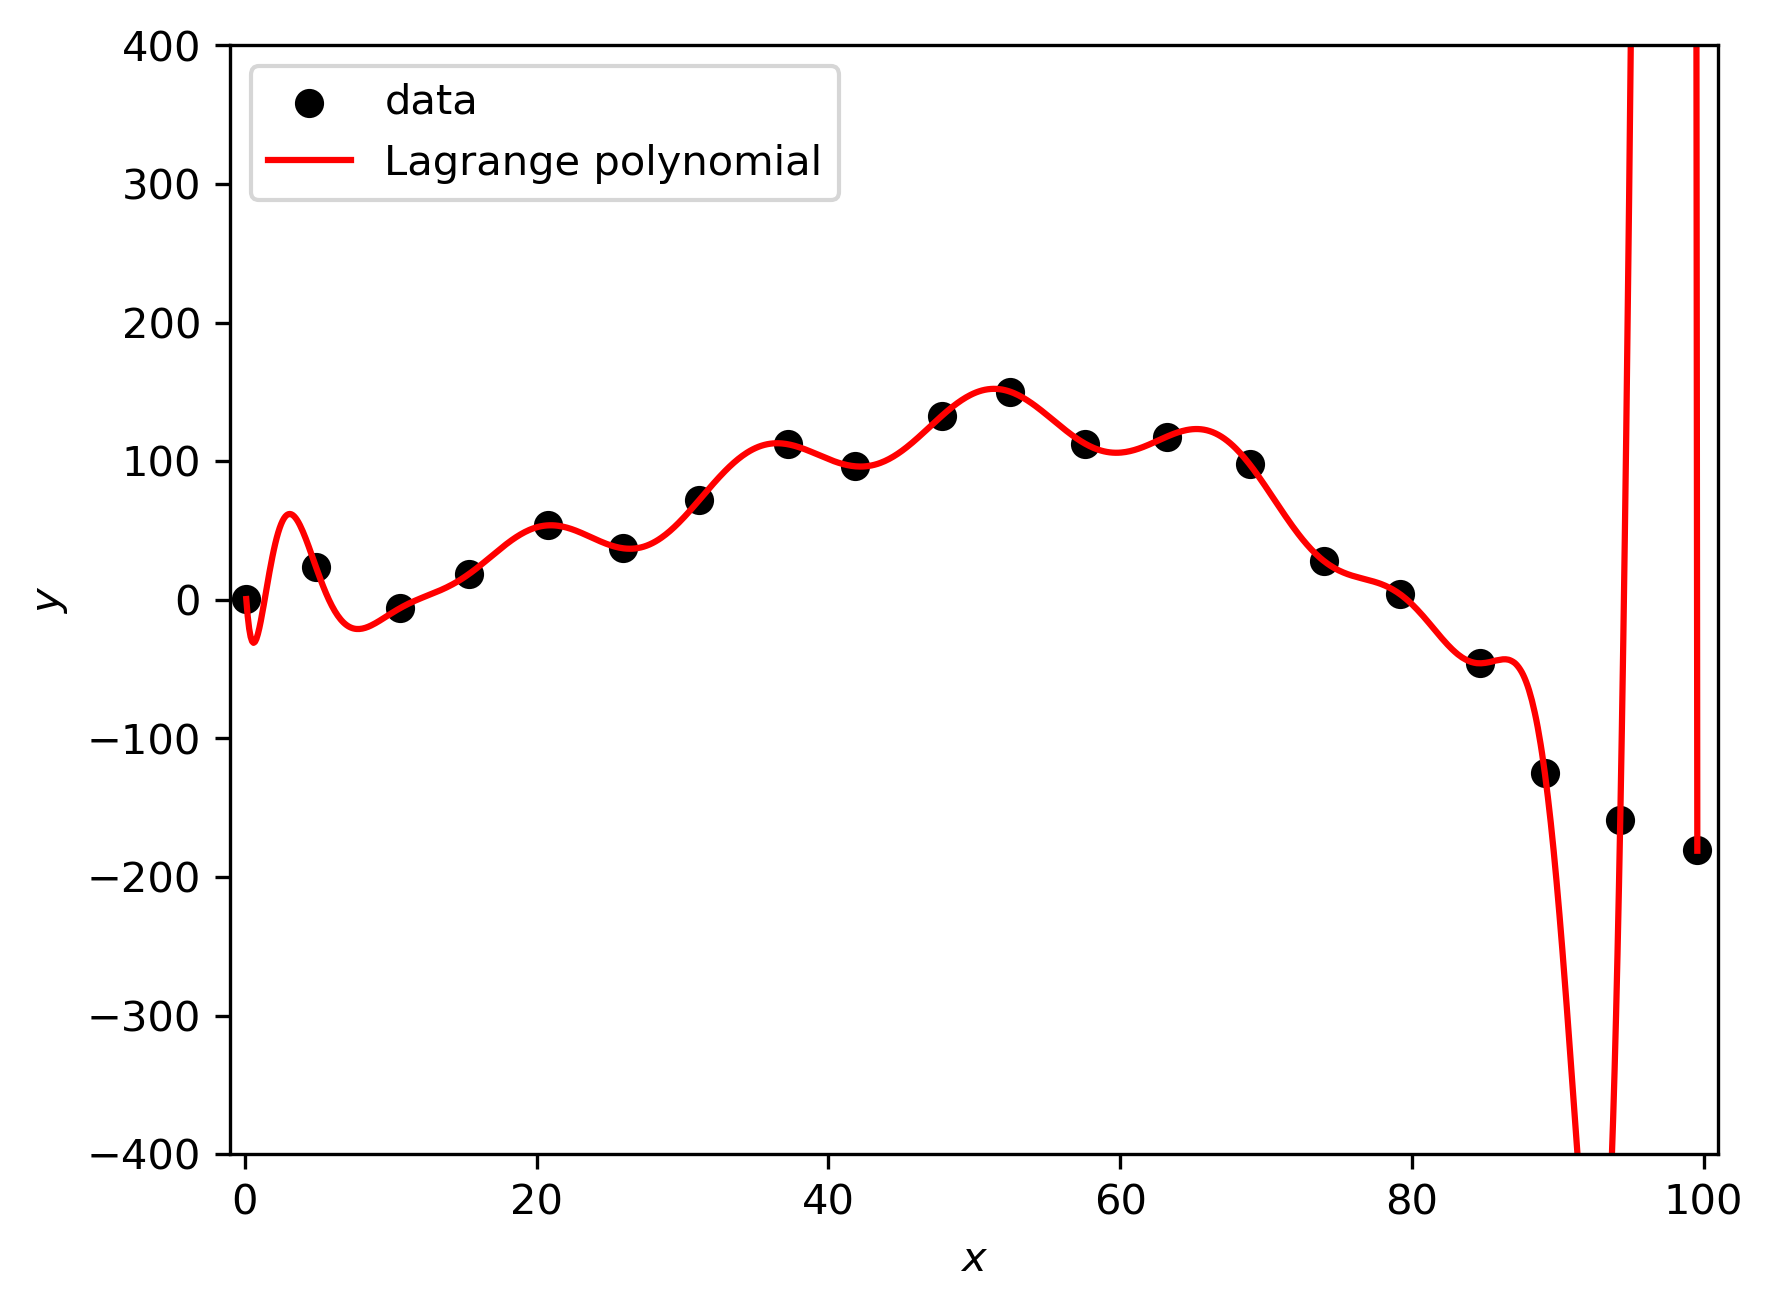
\includegraphics[width=0.75\linewidth]{./plots/vander_pol.png}
  \caption{The Lagrange polynomial with the original data points. To generate the polynomial we used the Vandermonde matrix. The system was solved using the LU decomposition method. We notice that the polynomial crosses all the points in our dataset.}
  \label{fig:van_pol}
\end{figure}

As we see in \Cref{fig:van_pol} the generated polynomial passes through all of our data points as we would expect. It is worth mentioning that for this example we use the full 19th order polynomial that can be generated using all 20 points of our data. However, this interpolation is not so useful as it greatly overfits our data. 

\begin{figure}[H]
  \centering
  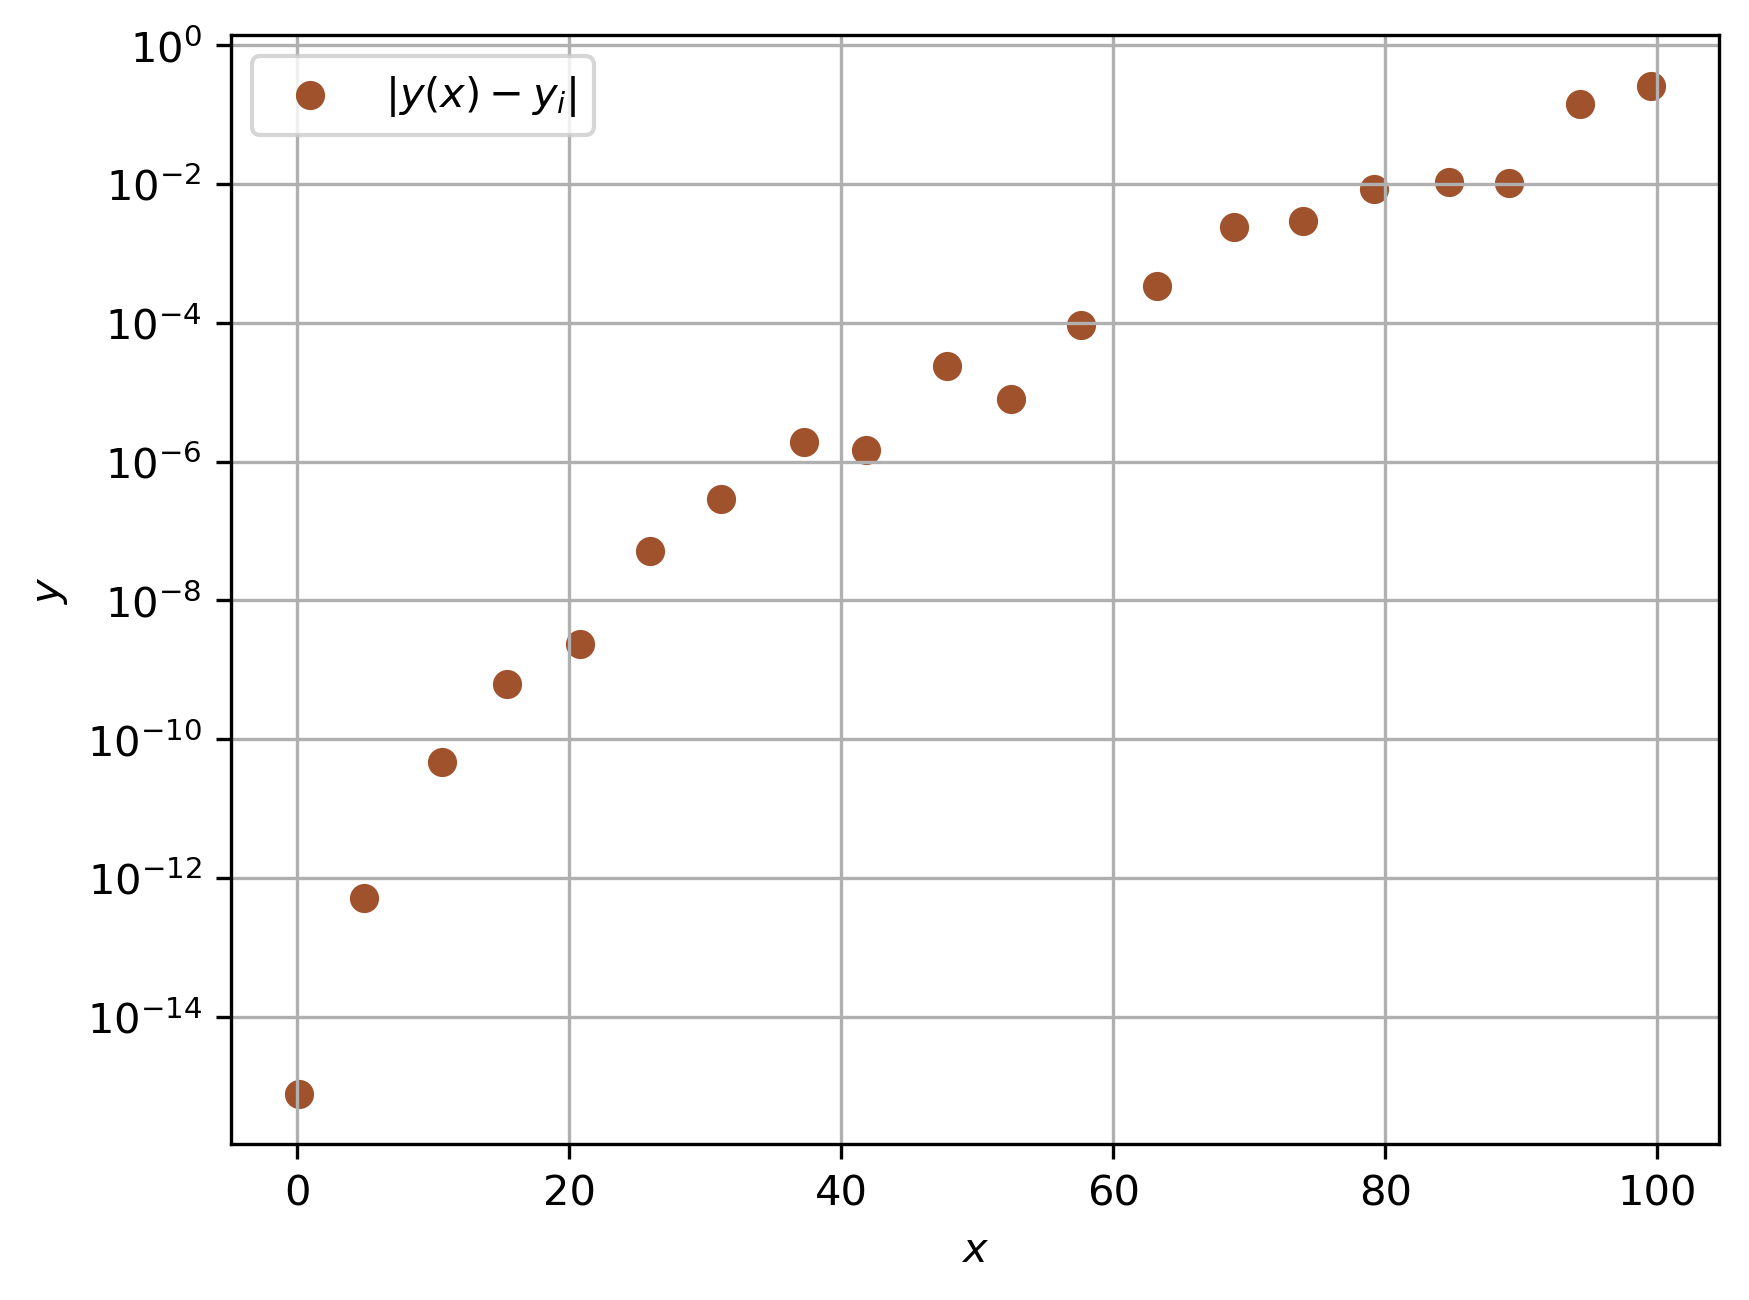
\includegraphics[width=0.75\linewidth]{./plots/vander_dif.png}
  \caption{The absolute difference between the actual and the interpolated values. To perform the interpolation we used the Vandermonde matrix and LU decomposition to solve the system. We see that the precision at the first points is great but gets increasingly worst for bigger values of $x$.}
  \label{fig:van_dif}
\end{figure}

In \Cref{fig:van_dif} we plot the absolute difference between the given points and the predictions at the same position $(x)$. By doing this we can check if the polynomial is lying exactly on top of our data. As we can see the polynomial is very accurate for the first few data points and gets increasingly less precise for the last points. Still, the deviation is smaller than $1$ while the range of our dataset is $[-180.8,150.2]$.  

\subsection{Neville’s Algorithm}
\label{chap:nev}

\lstinputlisting{neville.py}

We want to confirm that the polynomial we calculated in \Cref{chap:lu_dec} is the same as the Lagrange polynomial that we can find when applying Neville's algorithm. To do that we define a new function ``nevil'' that applies this algorithm on a set of points $(x\_true,y\_true)$. The input should also include the $x$ values we want to interpolate at and the degree of the outcome polynomial. 

The way the function works is that it finds $j\_low$ by using the bisection algorithm. The $j\_low$ variable keeps the position of the lowest of the $m$ nearest neighbors where $m$ is the degree of the polynomial $+1$. The function then initializes an array with the $m$ nearest neighbors and updates using two nested loops. The final value we will interpolate for each point is given by the updated value of the first position of the array. This process is repeated for every single point we want to interpolate for. 

In the main body of our script, we load our data as before and also apply the method we mentioned in the previous task (\Cref{chap:lu_dec}) to calculate the polynomial with the Vandermonde matrix. We then apply our ``nevil'' function for $n=\mathrm{len}(x)-1$ to find the full Lagrange polynomial and interpolate on the same $x$ values. We plot both polynomials with the original data points. We also plot the absolute difference between the interpolated and the real values as we did in the previous code. 

\begin{figure}[H]
  \centering
  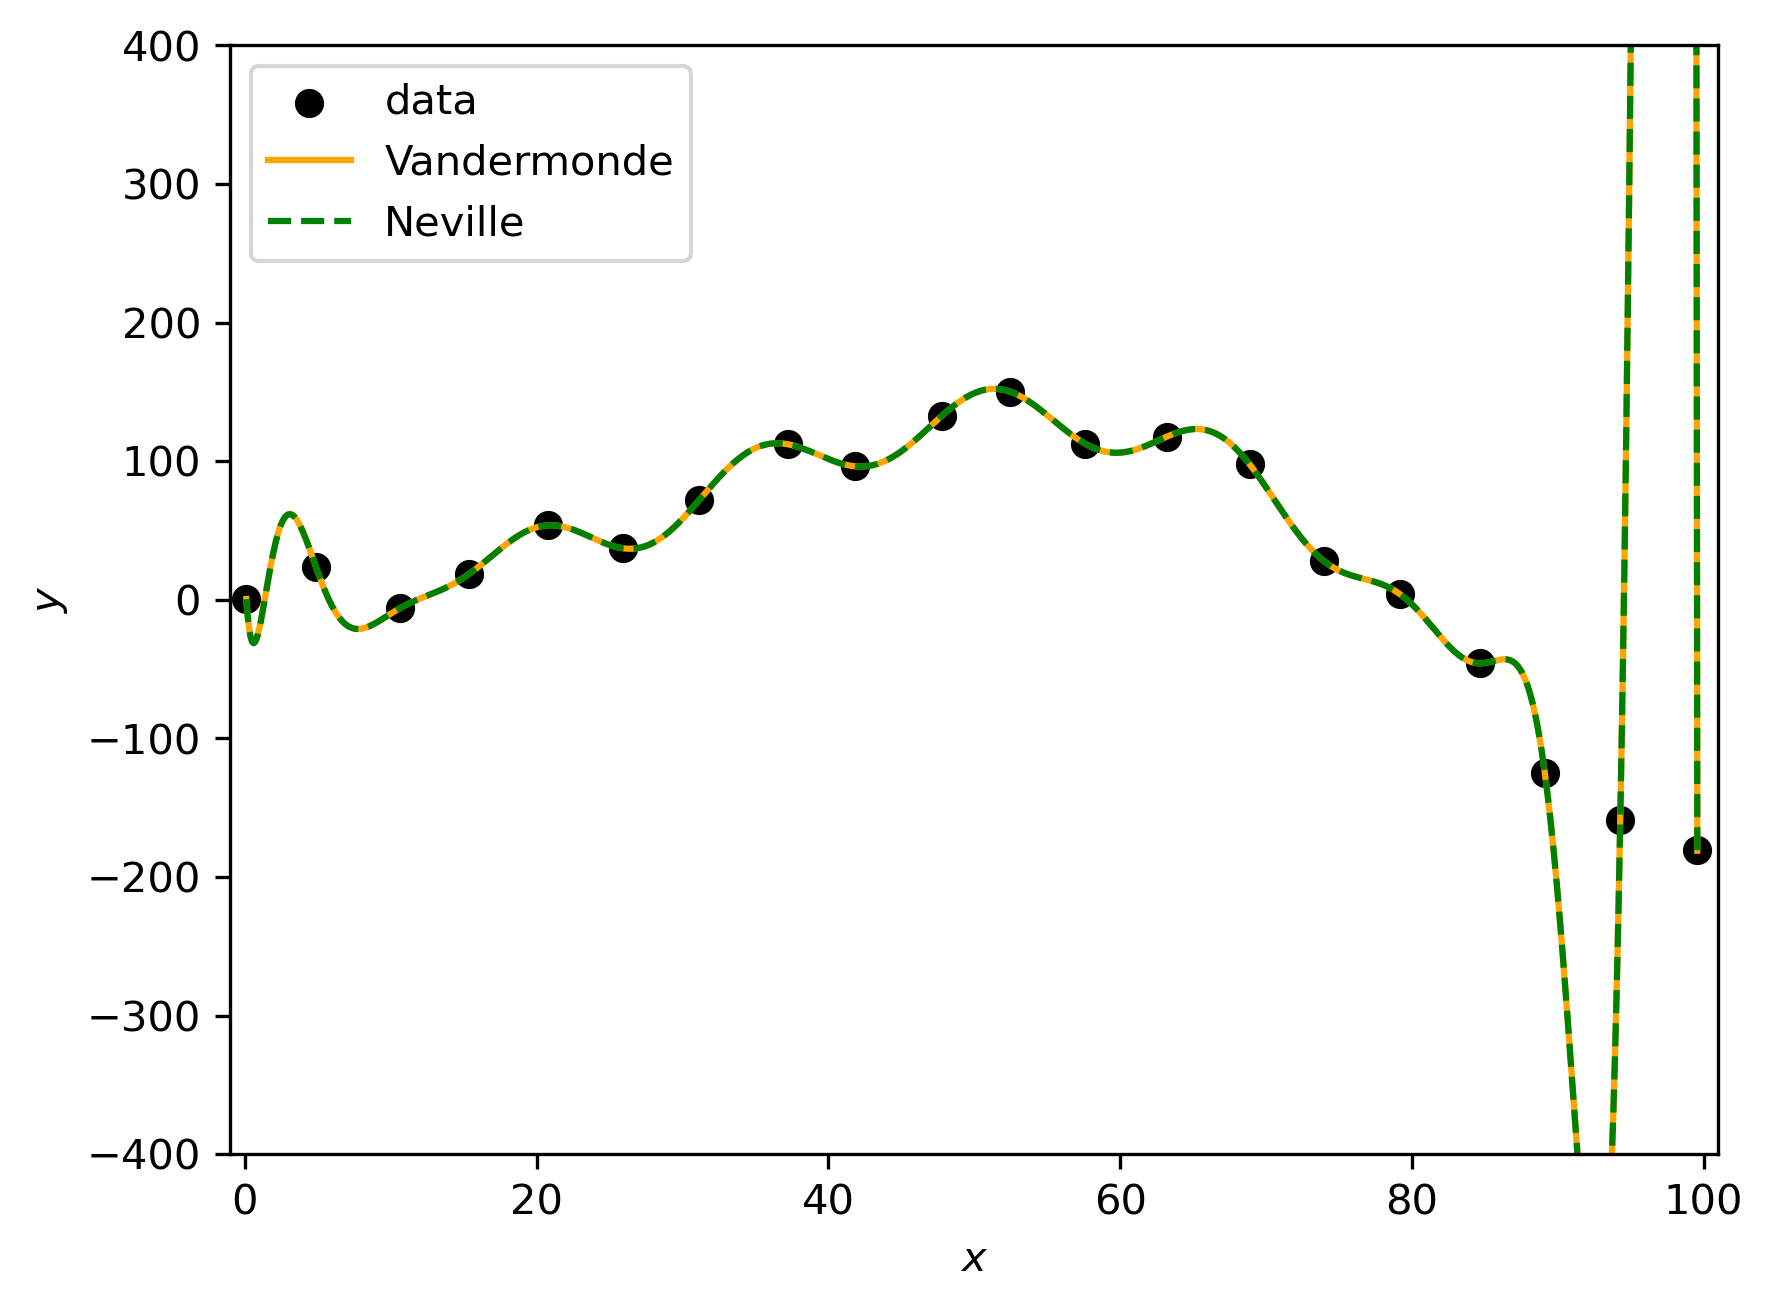
\includegraphics[width=0.75\linewidth]{./plots/compare.png}
  \caption{The data points with the full Lagrange polynomial that passes through them as it was calculated using two different approaches. With orange we show the method we implemented in \Cref{chap:lu_dec} that uses the Vandermonde matrix. With the dashed green line, we show Neville's method which we implemented for this task. We used a dashed line to show how both of the approaches give us the same polynomial as they fall on top of each other. }
  \label{fig:nev_pol}
\end{figure}

In \Cref{fig:nev_pol} we can see that the two different approaches to calculating the Lagrange polynomial give us the same solution as we would expect. The two plots lie on top of each other and pass through all the data points. In \Cref{fig:nev_dif} we have a closer look at the absolute difference between the interpolated (with Neville's algorithm) and the true values for all the points. We can achieve higher precision with this approach as these differences are smaller compared with \Cref{fig:van_dif} where we used the Vandermonde matrix.  

\begin{figure}[H]
  \centering
  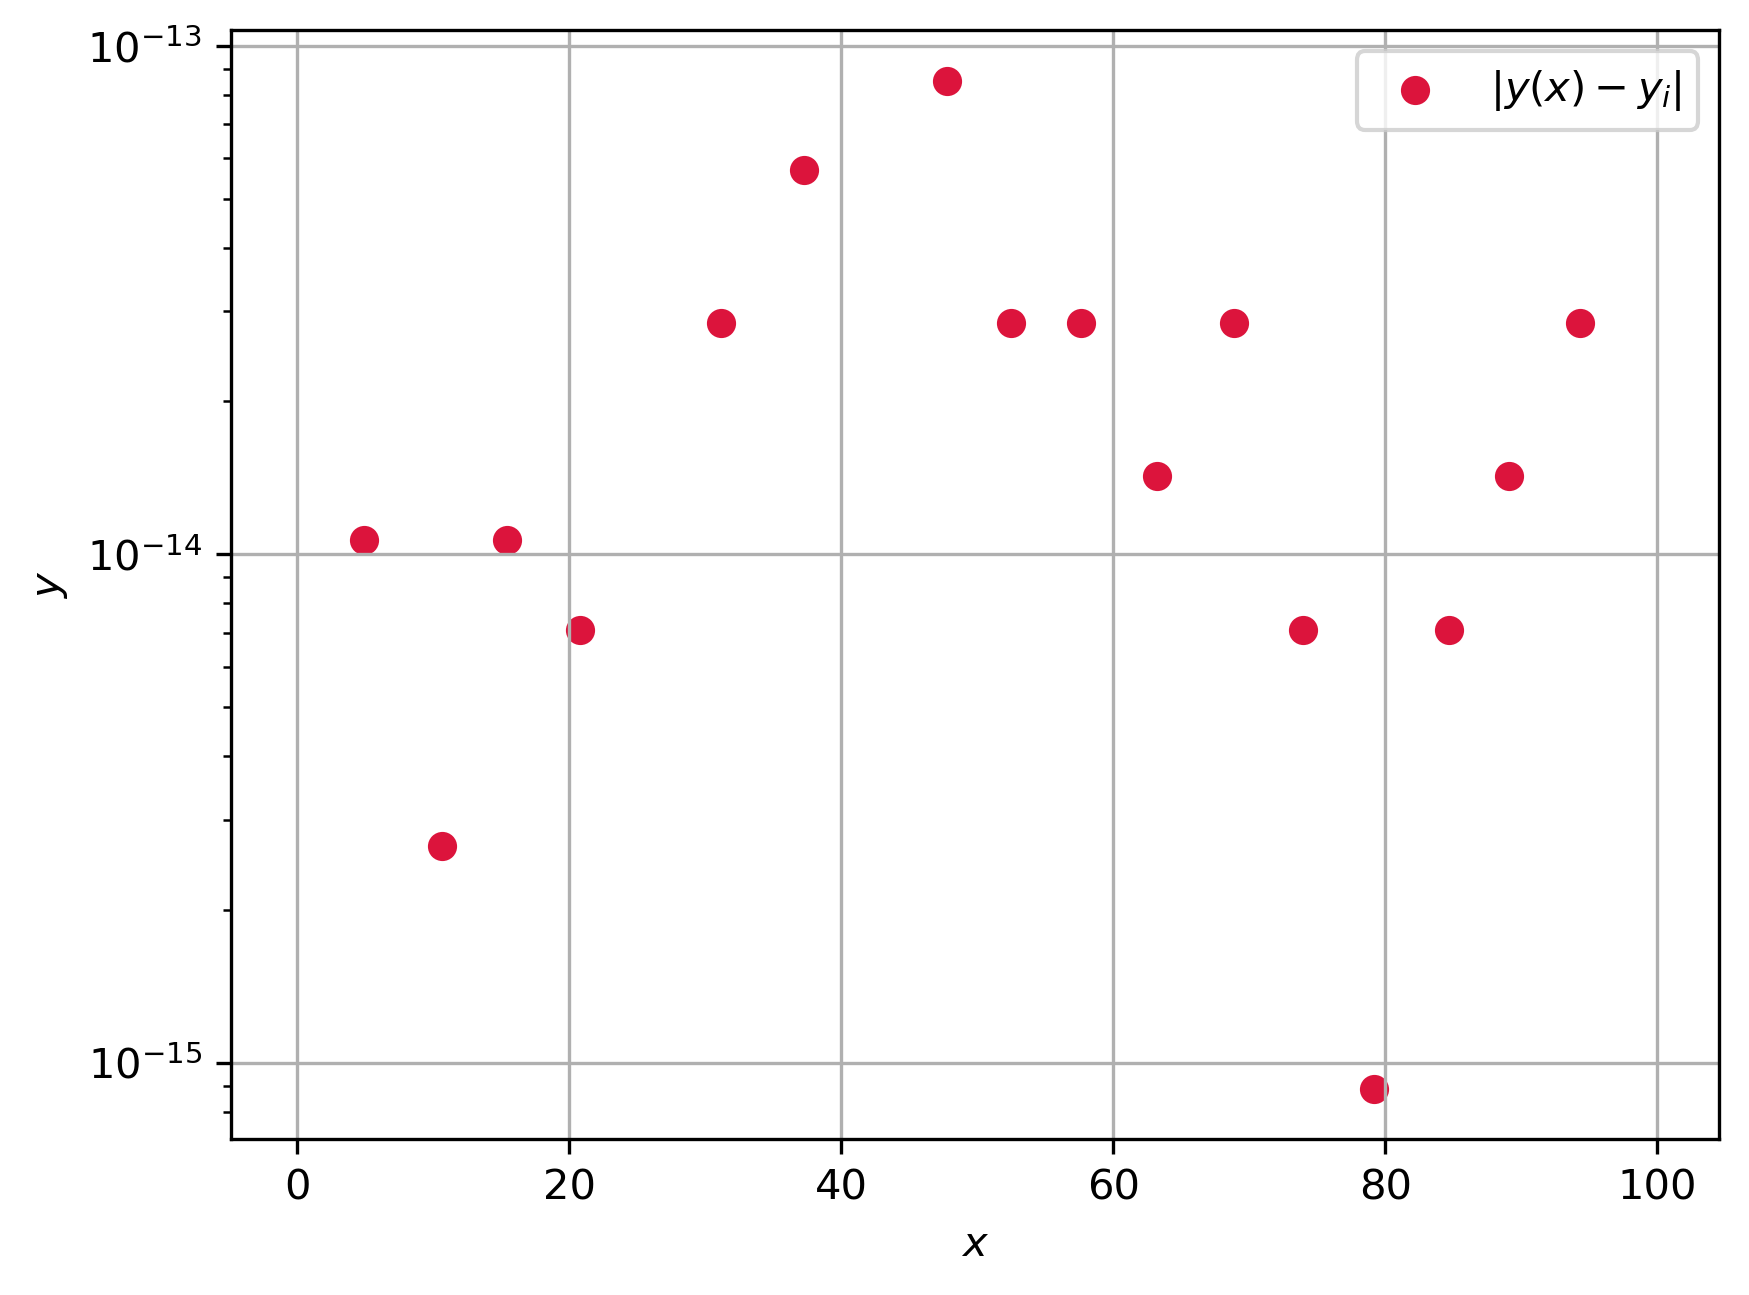
\includegraphics[width=0.75\linewidth]{./plots/nevil_dif.png}
  \caption{The absolute difference between the actual and the interpolated values. To perform the interpolation we used Neville's algorithm. We see that we managed to achieve great precision for all the data points.}
  \label{fig:nev_dif}
\end{figure}

\subsection{Iterative Improvements}
\label{chap:lu_iter}

\lstinputlisting{iteration_lu.py}

We now want to use the LU decomposition to iterate on the solution in an attempt to improve the results we got from the Vandermonde matrix method. To do that we create a new function ``lu\_iter'' that uses all the functions we used to get the interpolated results by using the Vandermonde matrix. For $n=1$ the function is finding the solution in the same way that was described in \Cref{chap:lu_dec}. For $n>1$ we have more iterations over our solutions by solving the system $L U \delta c = V c - y $ where $V$ is the Vandermonde matrix and $c$ the array with our initial solution. When we find $\delta c$ we can update our solutions by calculating $c_{new}=c - \delta c$

In our script, we simply use our function to generate the interpolated predictions using $n=1$ to get the results we had in \Cref{chap:lu_dec} and $n=10$ to get the new results for $10$ iterations. We also plot the absolute difference between the interpolated and the real values, this time for both $1$ and $10$ iterations at the same figure. 

In \Cref{fig:iter_pol} we can see how the two polynomials calculated for $1$ and $10$ iterations are on top of each other as we would expect. To distinguish between them we can look at \Cref{fig:iter_dif} where we have the absolute differences at the data points. We can say that increasing the number of iterations did not achieve better results as we would expect, but rather both approaches had the same deviations from the true values. 

\begin{figure}[H]
  \centering
  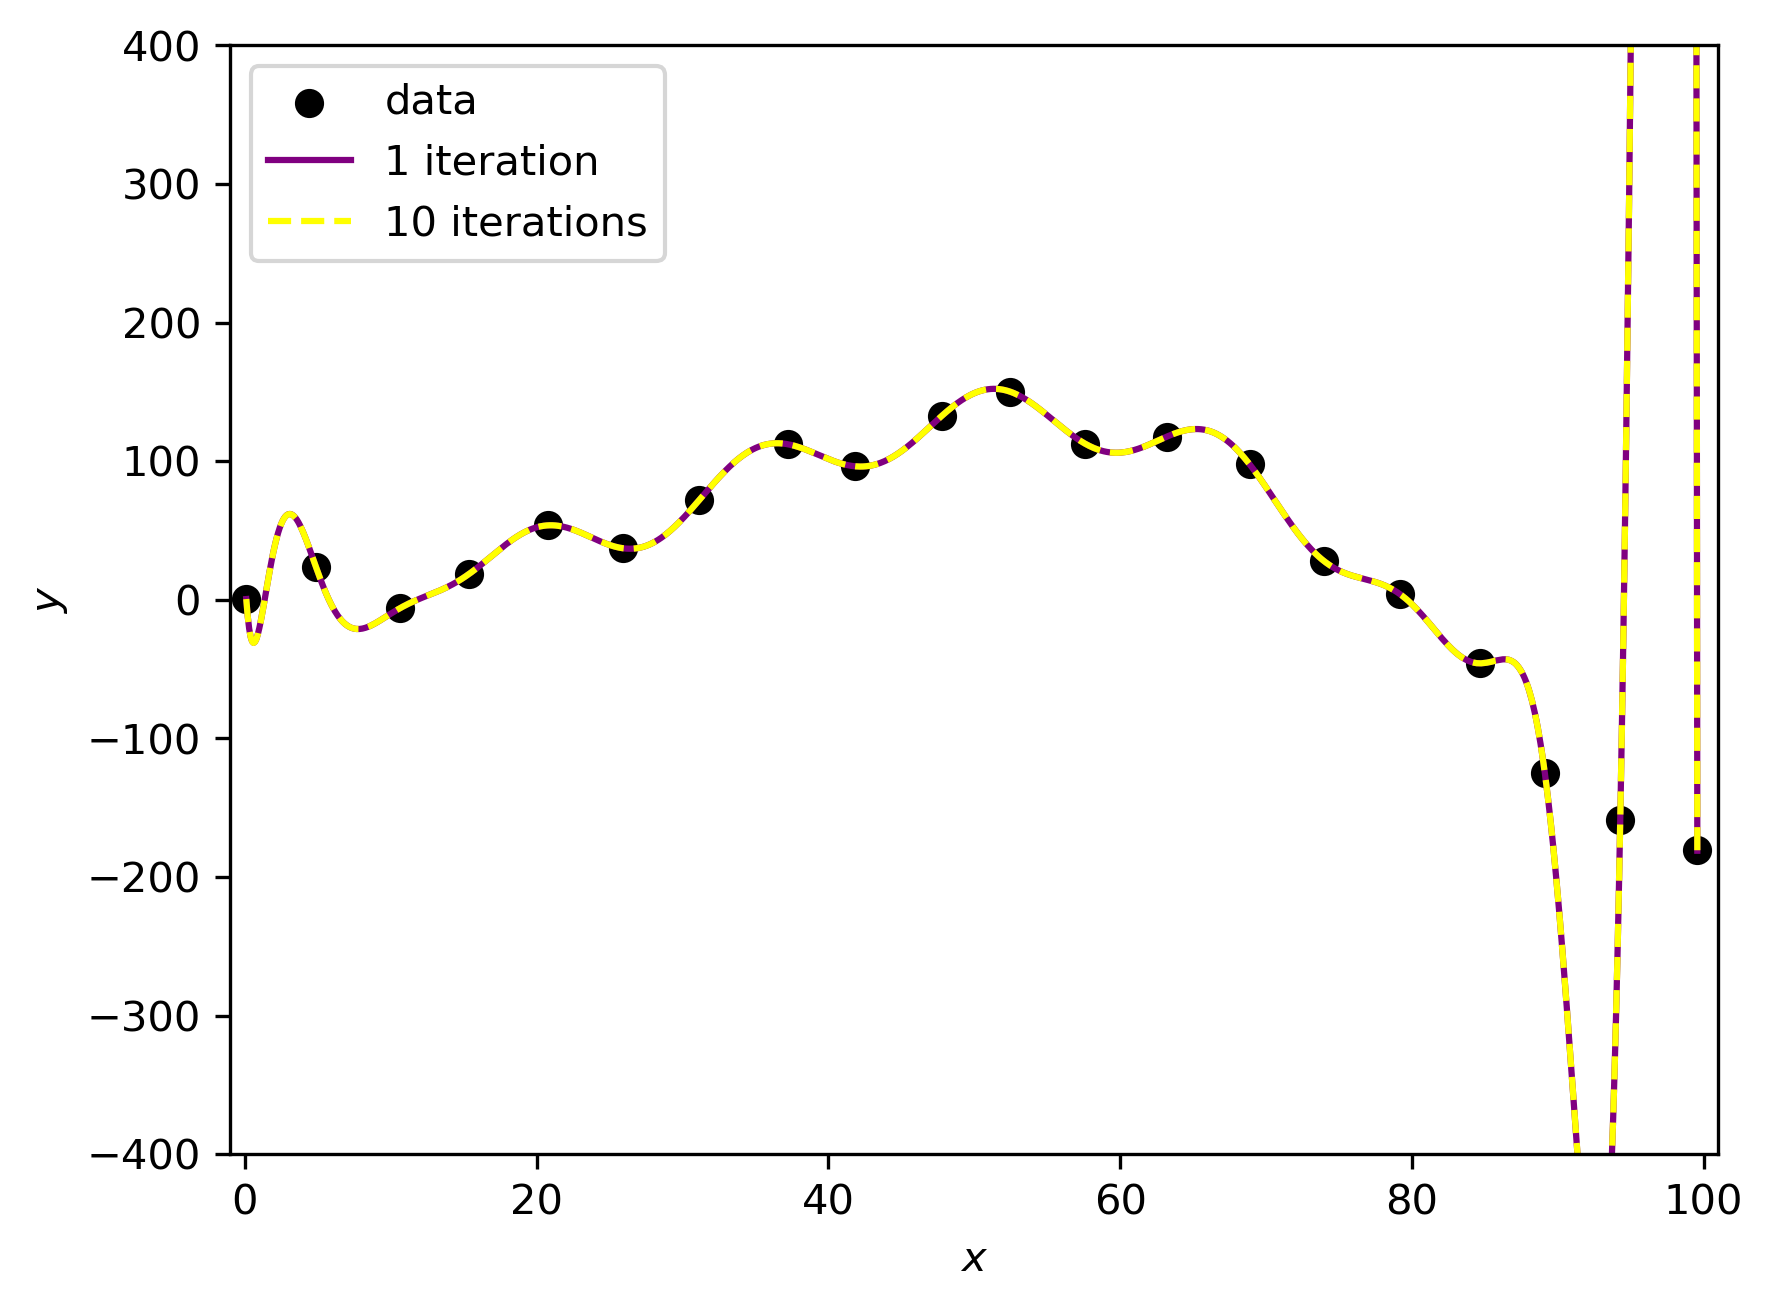
\includegraphics[width=0.75\linewidth]{./plots/iter_comp.png}
  \caption{The Lagrange polynomial with the original data points. To generate the polynomial we used the Vandermonde matrix. The system was solved using the LU decomposition method for $1$ (purple) and $10$ (yellow) iterations. We notice that the polynomials fall on top of each other and cross all the points in our dataset.}
  \label{fig:iter_pol}
\end{figure}

\begin{figure}[H]
  \centering
  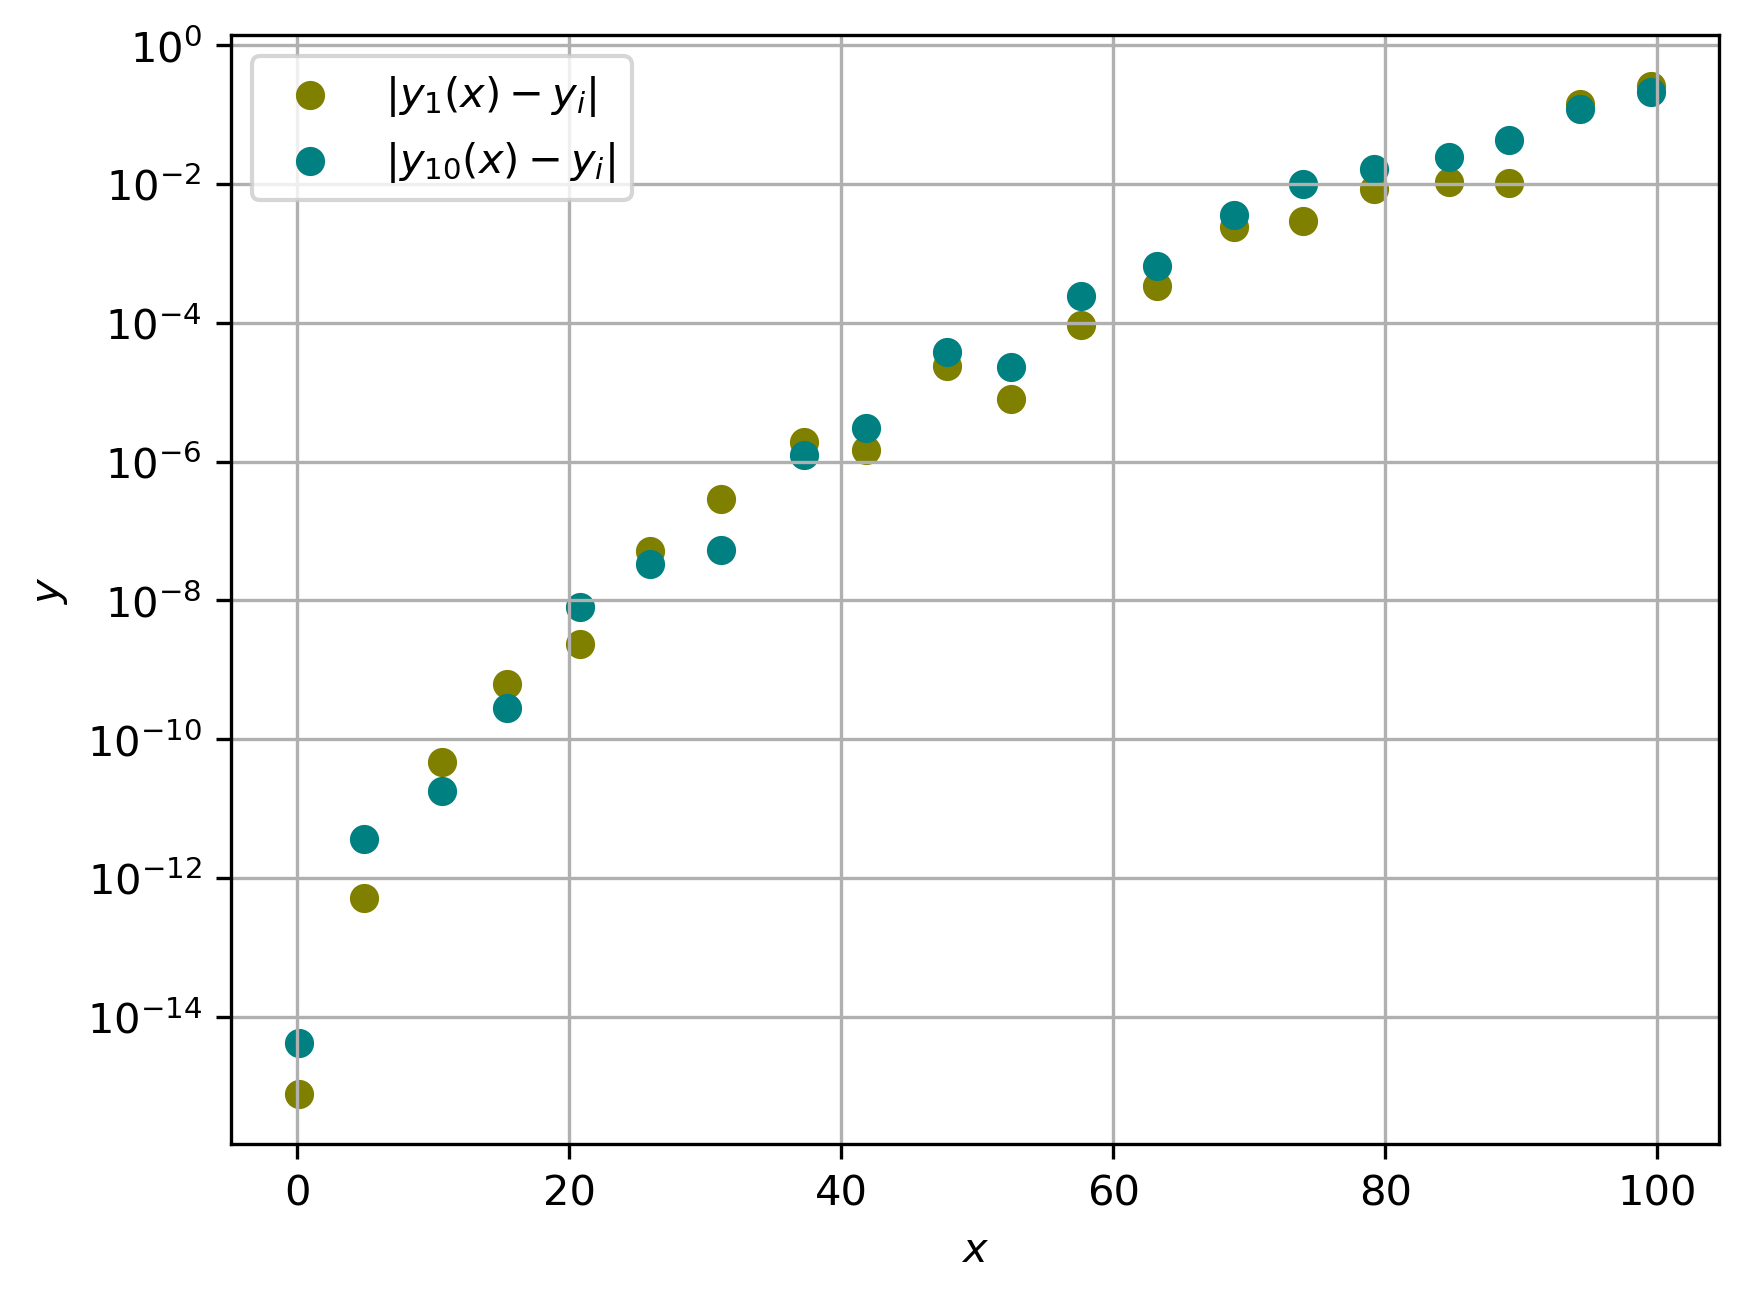
\includegraphics[width=0.75\linewidth]{./plots/iter_dif.png}
  \caption{The absolute difference between the actual and the interpolated values. To perform the interpolation we used the Vandermonde matrix and LU decomposition to solve the system with $1$ iteration (green) and $10$ iterations (blue). For both approaches the precision at the first points is great but gets increasingly worst for bigger values of $x$. The increased number of iterations did not yield better precision.}
  \label{fig:iter_dif}
\end{figure}

\subsection{Timing all executions}

\lstinputlisting{time_1.py}

In this final task, we want to time the three methods we developed in this section. To achieve that we use the ``timeit'' module. When we call the ``timeit'' function of that module we can specify the number of repetitions and we also need to import all the necessary functions and data. We will time the ``nevil'' function from \Cref{chap:nev} and the ``lu\_iter'' function from \Cref{chap:lu_iter} for $n=1,\:10$ to get the time for $1$ and $10$ iterations. We are interested in finding the time needed for $100$ repetitions of each algorithm. Because ``lu\_iter'' is much faster we can run it for $1\,000$ repetitions and divide the result by $10$ to make our results more accurate. 

\lstinputlisting{output/time_1.txt}

The output of our code shows the time needed for 100 repetitions of each of the methods we used to calculate the Lagrange polynomial in this assignment. 

The difference in the execution time comes from the way these algorithms operate and were implemented. For Neville's algorithm, we use two nested loops to update an array for each of the points we wanted to interpolate. All these loops are very costly in terms of execution time. The LU decomposition of the Vandermonde matrix is implemented with only a single loop and uses matrix multiplications to perform all the calculations. This is the reason it is much faster than Neville's algorithm. The slowest part of the function ``lu\_iter'' is executing the ``predict\_vander'' function that generates the predictions after we calculated the array of the coefficients. This is the reason why increasing the number of iterations is not affecting the execution time that much, because the predictions are generated once regardless of the number of iterations.

To determine which one should give us the most accurate results we need to compare \Cref{fig:nev_dif,fig:iter_dif}. As we already discussed, increasing the number of iterations did not improve our results. Neville's algorithm gives us the best results for the whole set of points and can therefore be considered the most accurate implementation for the Lagrange polynomial. 

\begin{figure}[H]
  \centering
  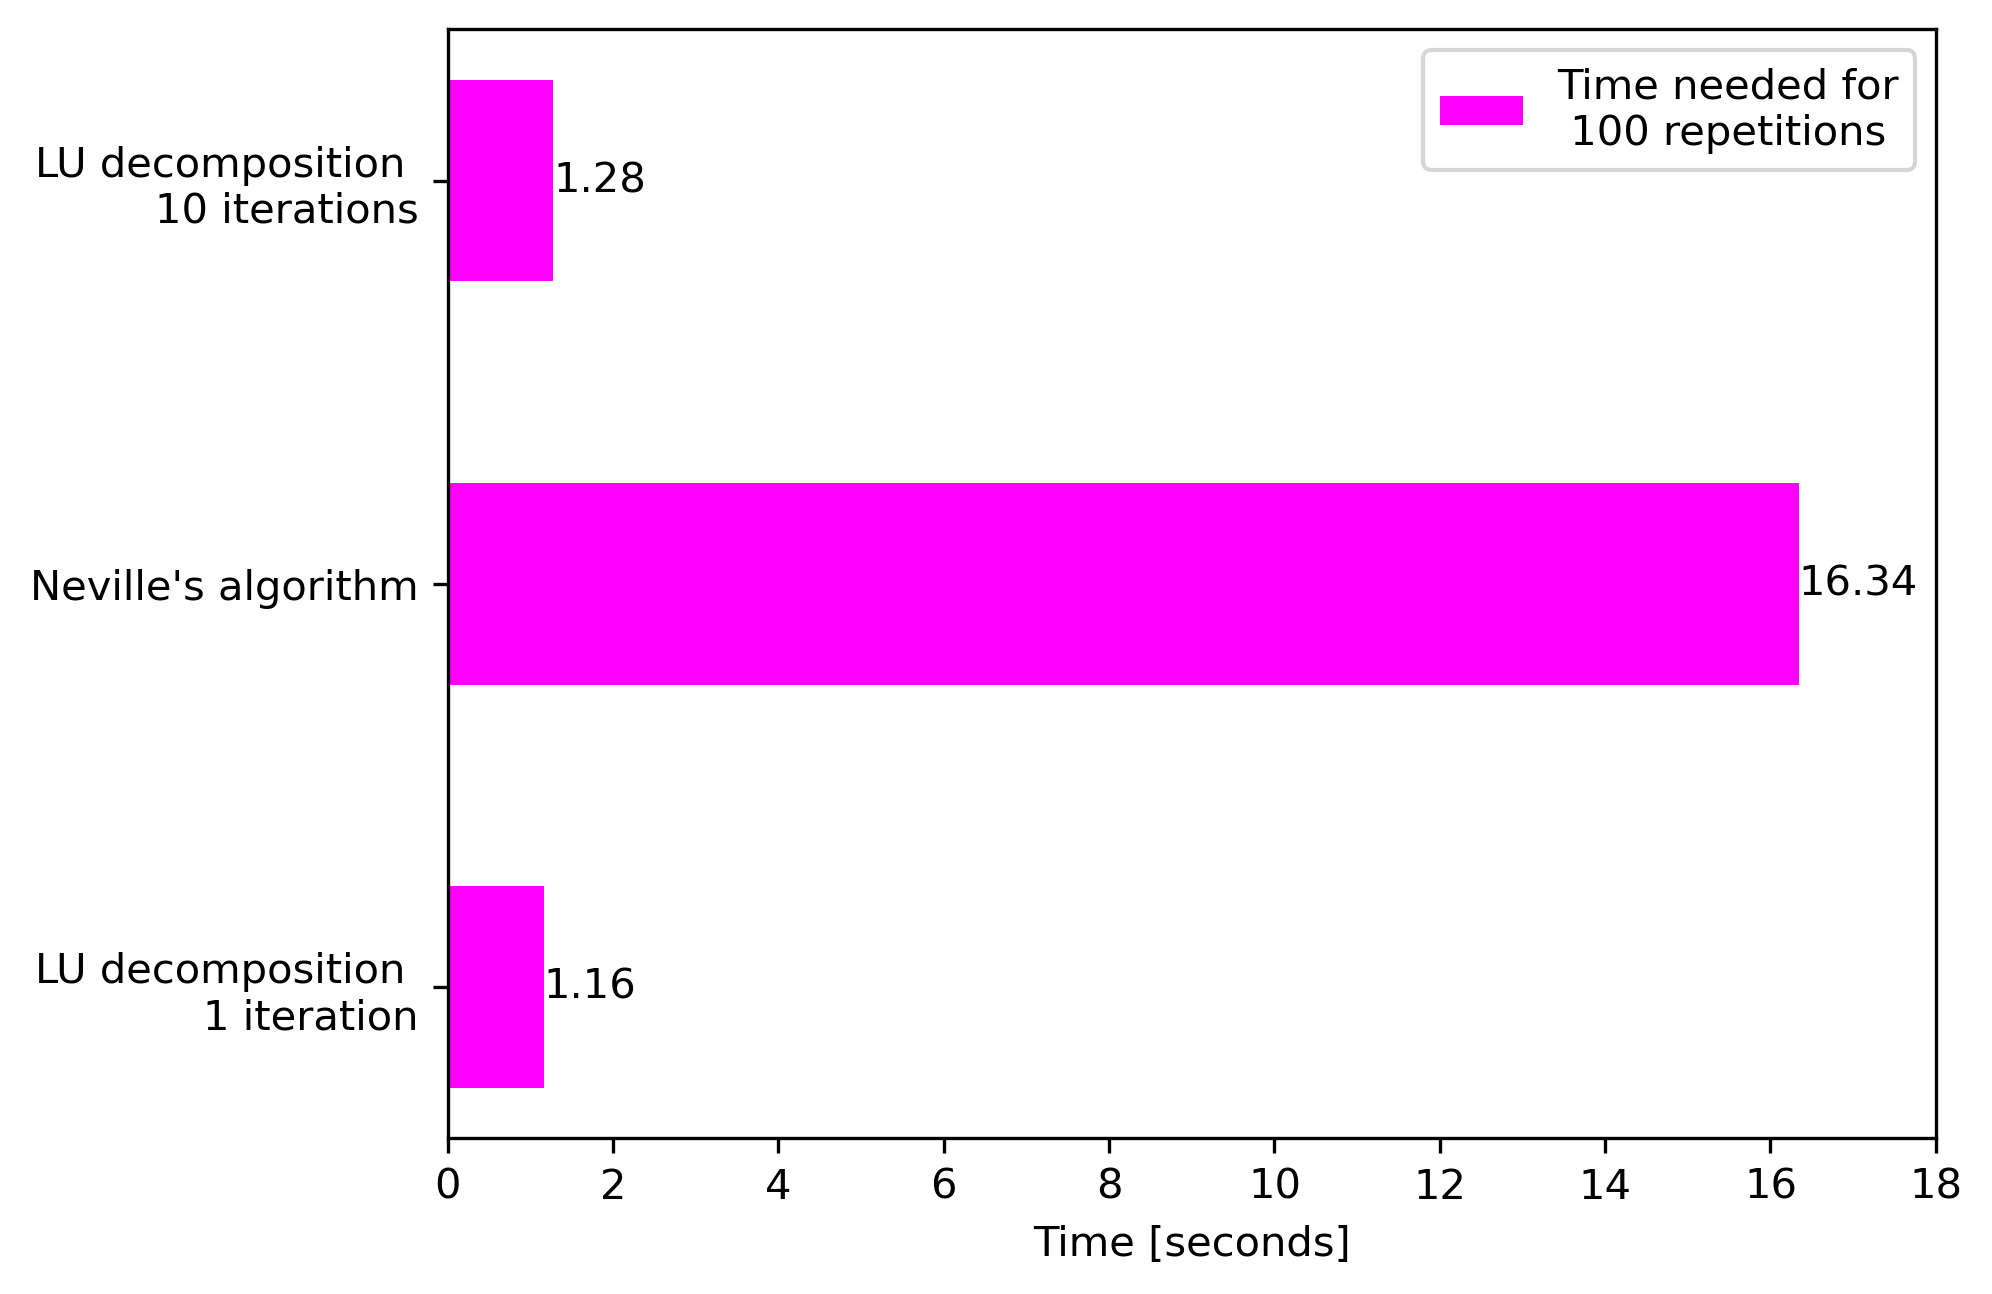
\includegraphics[width=0.75\linewidth]{./plots/time.png}
  \caption{ The time needed for 100 repetitions of each of the methods used to calculate the Lagrange polynomial. Neville's algorithm was much slower than the Vandermonde matrix with the LU decomposition. Increasing the number of iterations leads to only a small increase in the execution time.  }
  \label{fig:time}
\end{figure}

\end{document}
